\fancychapter{Background}

In this section, we will start by generally describing what clustering is and how it works. We will then outline how ~\ac{SOM}~\cite{Kohonen1990} perform, which is the document clustering algorithm used on this thesis.

\section{Document Clustering}
\label{sec:clustering}
Document clustering is an optimal division of documents into categories without prior knowledge of the data that is being organized, based only on the similarity between them. Due to the fact that no prior knowledge of the data has to be known, document clustering is labeled as Unsupervised \ac{ML}~\cite{hinton1999unsupervised}.

~\citet{Liu2012b} asserted that document clustering can be used in a variety of Computer Science fields, such as:
\begin{itemize}
  \item Natural Language Preprocessing.
  \item Automatic Summarization.
  \item User preference mining.
  \item Improving text classification results.
\end{itemize}

There are two main types of document clustering: hard clustering and soft clustering. In hard clustering, one document can only belong to one cluster, while in soft clustering one document can belong to multiple clusters. 

%REMOVEDBYPAVEL
%In regard to document categorization~\citet{Springorum1998} performed clustering with SOMs~\citep{Kohonen1990} while identifying polysemous German Propositions. They used regular SOMs to create multiple clusters and used Centroid-Based or Preposition-based softening to create Soft Clusters from the Hard Clusters.

The clustering process usually works as described in Figure~\ref{fig:1_Text_Clustering_Main_Framwork}. In the first step, a data set must be provided with the documents to be clustered. The second step is where non relevant words are removed from the documents, to improve clustering quality~\cite{Kang2003}. 

\begin{figure}
  \begin{center}
    \includegraphics[width=12cm]{images/1_Text_Clustering_Main_Framwork.png}
  \end{center}
  \caption{ Text clustering main framework~\cite{Dozono2012} }
  \label{fig:1_Text_Clustering_Main_Framwork}
\end{figure}

%REMOVEDBYPAVEL
%Another way to extract keywords is to differentiate text features by analyzing the document corpora. For example if the dataset is composed from HTML or XML documents it is possible to identify more relevant features due to the characteristics of the document syntaxe.
The third step is characterized by converting the keywords of each document into vectors. The most common model used for this task is \ac{VSM}. In \ac{VSM}, each vector dimension represents one detected keyword and each document is represented by the vector of keywords in the feature space. This process is illustrated in Figure~\ref{fig:2_svm} and works in the following way:
\begin{itemize}
  \item \textbf{First step:} string tokenization, and token selection. In this case, stop words and repeated words will be removed.
  \item \textbf{Second step:} string to \ac{VSM} conversion. Each different word will correspond to a position in the array, and its value will correspond to the number of occurrences. 
\end{itemize}

\begin{figure}
  \begin{center}
    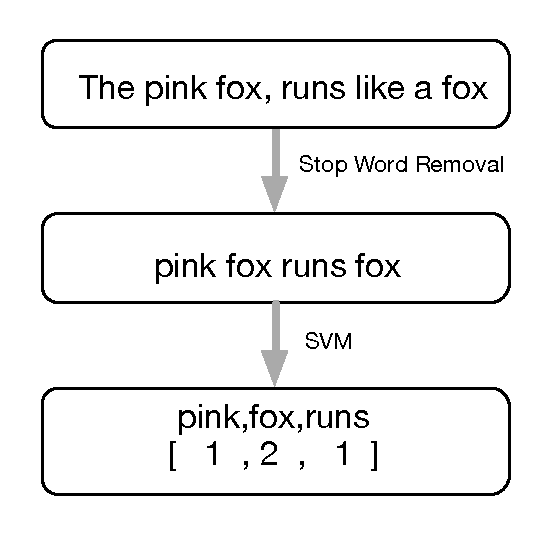
\includegraphics[width=5cm]{images/2_svm.eps}
  \end{center}
  \caption{ Text tokenization and transformation to Vector Space Model. }
  \label{fig:2_svm}
\end{figure}

There are many clustering algorithms. In the following section we will describe the particullar case of the \ac{SOM} algorithm, the solution used in our work.

\section{The Self-Organizing Map} 
\label{sec:the_self_organizing_map}

\ac{SOM} are a two layer recurrent \ac{ANN} that has the desired property of topology preservation, thus mimicking the way the cortex of highly developed animals brains work. \ac{SOM} allow cluster visualization of multi-dimensional data, similar to methods such as \ac{MDS}~\cite{KruskalWish1978} and \ac{PCA}~\cite{Hotelling_1933} .  

\citet{Bacao2005} described the basic idea behind \ac{SOM} as a mapping between input data patterns into a n-dimensional grid of neurons, or units. That grid is also know as the output space, as opposed to the initial space --- input space --- where the input patterns reside. An illustration of both spaces can be seen in Figure~\ref{fig:5_neighbours_converge}.

SOMs work in a similar way as is thought the human brain works. Analogously to the human brain, SOMs also have a set of neurons that, through learning experience, specialize in the identification of certain types of patterns. These neurons are responsible for categorizing the input patterns for which they are responsible to identify. Nearby neurons will be organized by similarity, which will cause similar patterns to activate similar areas of the \ac{SOM}.
With this topology preserving mapping, the \ac{SOM} organizes information spatially, where similar concepts are mapped to adjacent areas. The topology is preserved in a sense that, as far as possible, neighborhoods are preserved throughout the mapping process.
Output neurons are displayed in an N dimensional grid, generally rectangular, but other structures are possible, such as hexagonal or octagonal.  The grid of neurons, in the output space, can be divided in neighborhoods --- where neurons responsible for the same kind of input reside.
In \ac{SOM}, neurons will have the same amount of coefficients as the input patterns and can be represented as vectors.

Before describing the algorithm, it is important to define two key aspects of the \ac{SOM}: the learning rate and the quantization error. The learning rate is a function that will be decreased to converge to zero. It will be applied to winning neurons and their neighbors in order for them to move toward the corresponding input pattern in progressively smaller steps. Quantization error is the distance between a given input pattern and the associated winning neuron. It describes how well neurons represent the input pattern. The radius of the neighborhood around the winning neuron is also particularly relevant to the topology of the \ac{SOM}, deeply affecting the unfolding of the output space as stated by~\citet{Bacao2005}. 

SOM training is always subject to some variability due to multiple causes, like the sensitivity of initial conditions, convergence to local minima and sampling variability~\cite{Bodt}.

No general formula exists to minimize quantization error~\cite{Bodt} . In order to achieve a minimal value, the number of neurons, value of neurons and order of the input data is randomly changed. Multiple SOMs are trained and the one with the lowest mean quantization error is chosen.

In order to know how well a neuron maps to all the input patterns it represents, the average of the quantization error can be used(Eq. \ref{eq:avg_quant_error}). On the equation, $d_{i,n}$ is an input pattern that is represented by the neuron $w$. Each neuron represents an arbitrary number --$n$--of input patterns, that group of input patterns is represented as $D_{i,j}$.
\par
\begin{equation}
  \label{eq:avg_quant_error}
  \varepsilon(w) = \frac{\sum_{i=0}^{n} \| w - d_{i}  \| }{n}, d_{i} \in D, \forall n
\end{equation} 


\input{./algorithms/som.tex}


\begin{figure}
  \begin{center}
    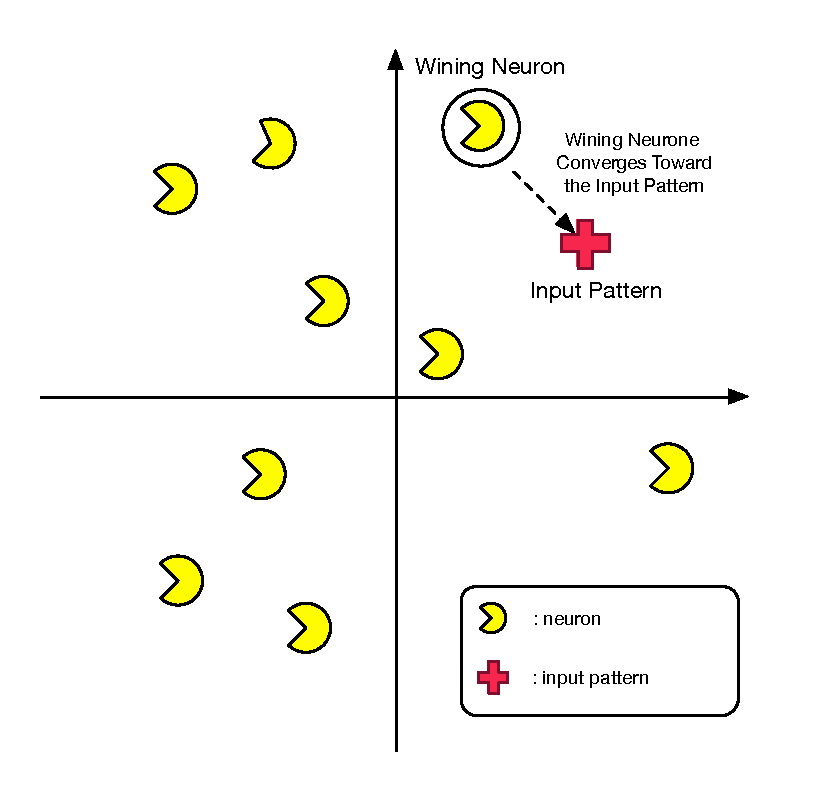
\includegraphics[width=5cm]{images/4_wining_neuron_converge.eps}
  \end{center}
  \caption{ Winning neuron converging at learning rate }
  \label{fig:4_wining_neuron_converge}
\end{figure}

\begin{figure}
  \begin{center}
    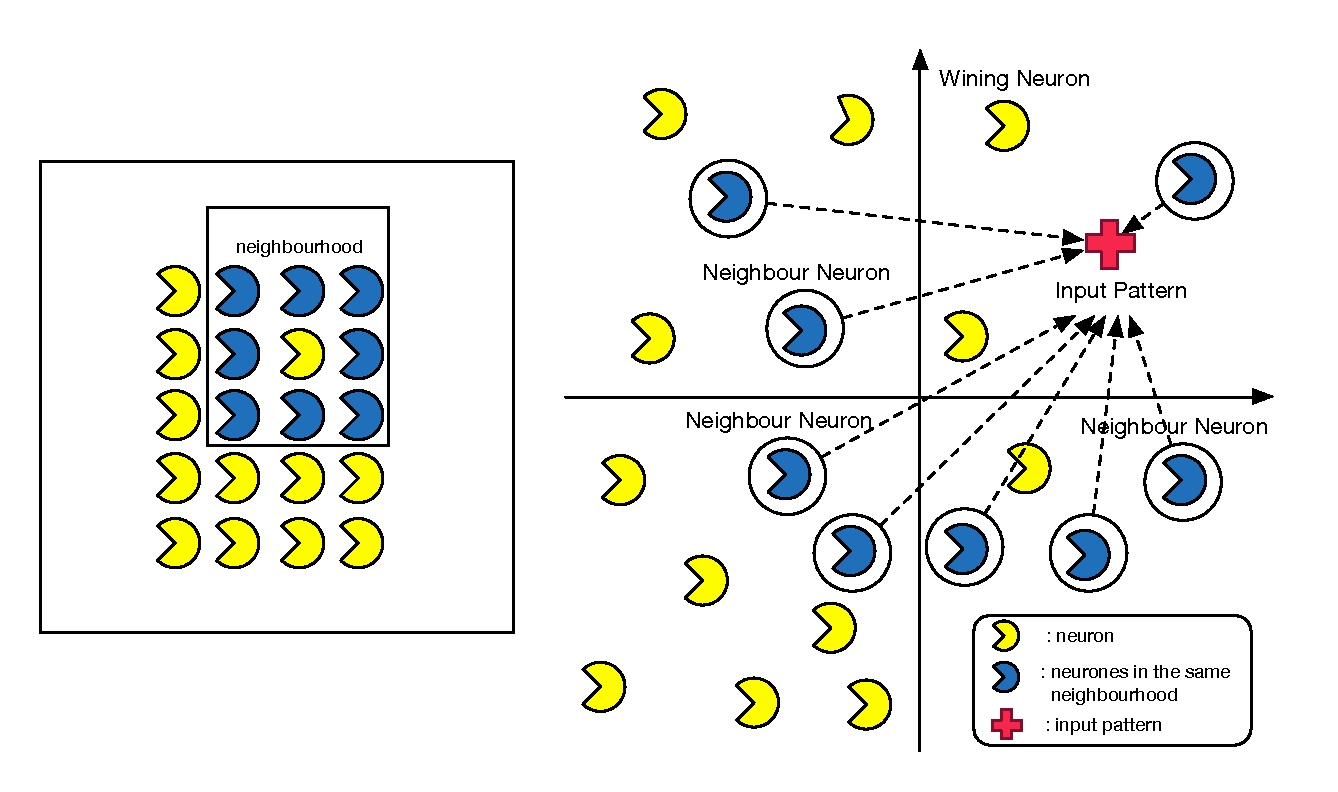
\includegraphics[width=12cm]{images/5_neighbours_converge.eps}
  \end{center}
  \caption{ On the left the output space neighborhood, on the right the neighbors of the winning neuron converging in the direction of the input pattern }
  \label{fig:5_neighbours_converge}
\end{figure}

The prediction phase can start after the model is learned. On the prediction phase, new input patterns can be quickly assigned to the \ac{SOM}, without need to apply the learning rate to the winning neuron and his neighbors. In other words, only line~\label{som:one} will run. Due to the fact that the input pattern will be assigned to the cluster that is mapped by the nearest neuron. Thus, it is very easy and fast to classify new data now. As stated by ~\citet{Liu2012b}, the advantages of using \ac{SOM} are: data noise immunity, easy to visualize data, and parallel processing.

In order to visually interpret the result of the \ac{SOM}, \ac{U-Matrix} method may be used~\citep{Bacao2005}. The \ac{U-Matrix} is a representation of the \ac{SOM}, in which, the distance between neurons is represented in a gray-scale where the darkest colors represent the farthest distance and the lightest colors the closer neurons. One way to compute the \ac{U-Matrix} is described in~\ref{alg:umatrix}. 

\begin{figure}[h]
  \begin{algorithm}[H]
    \label{alg:umatrix}
    \DontPrintSemicolon
    \KwData{$W = \{  \overrightarrow{w_{0,0}}$,\dots,$\overrightarrow{w_{n,n}}$ \} are the trained neurons 

            $D_{i,j}$ be the input patterns represented with neuron $w_{i,j}$

            $U$ is an empty matrix with size $2n-1.2n-1$
  }
    \KwResult{U-Matrix}
    \tcc{Initialize $U$ by adding the trained neurons}
    \For{ $w_{ij} = \overrightarrow{w_{00}}$ to $\overrightarrow{w_{n,n}}$ }{
      $U_{i*2, j*2} \leftarrow w_{i,j}$
    }
    \tcc{Calculate the distance between every adjacent neurons, and apply it to the square between them}
    \For{ $i=0$ to $U_{max}$}{
           
      \For{  $j=0$ to $U_{max}$}{
        
        \If{$l+1<m || j+1<m$}{
          $U_{i+1, j} = \| u_{i,j} - u_{i+2,j} \| $
          $U_{i, j+1} = \| u_{i,j} - u_{i,j+2} \| $
          $U_{i+1, j+1} = \frac{\| u_{i,j} - u_{i+2,j+2} \| + \|u_{i+2,j} - u_{i,j+2} \| }{2}$

        }
        $ j \leftarrow j + 1 $
      }
      $ i \leftarrow i + 1 $
    }
    \tcc{Substitute the neurons for an average of surrounding distances}
    \For{ $i=0$ to $U_{max}$}{
      \For{  $j=0$ to $U_{max}$}{
        $ u_{ij} = avg( Adj[u_{ij}] )$

        $ j \leftarrow j + 1 $
      }
      $ i \leftarrow i + 1 $
    }
    \tcc{convert the distances to color}
    $WHITE = 255$

    $BLACK = 0$

    $ u_{max} \leftarrow max(U) $

    $ u_{min} \leftarrow min(U) $

    \For{ $u_{ij} = u_{00}$ to $u_{n,n}$ }{
      $U_{i, j} \leftarrow (1 - \frac{ u_{i,j} - u_{min}  }{u_{max}-u_{min}})* WHITE$
    }
    \caption{U-Matrix }
  \end{algorithm}
\end{figure}


The \ac{U-Matrix} algorithm ( Alg.~\ref{alg:umatrix} ) is composed by four main cycles, which work in the following way:

\begin{itemize}
  \item \textbf{Cycle 1: } On line~\ref{um:initialize} neurons are added to the empty matrix, in order to be able to calculate the distance between them.
  \item \textbf{Cycle 2:} From line \ref{um:distance_h} to \ref{um:distance_d}, we are calculating the distance between adjacent neurons, and adding the distance to the empty position between them. On line \ref{um:distance_h} and line \ref{um:distance_v} we are looking for neurons horizontally and vertically, respectively. On line \ref{um:distance_d} we are looking for neurons on the diagonal. The diagonal calculus is more complex due to the fact that we need to calculate the lower diagonal to the current neuron, and average it withe the upper diagonal of the neuron immediately billow it.
    \item \textbf{Cycle 3: }At this stage the matrix is full of the distances between neurons, theoretically nothing else would be needed to be calculated. But it still has neurons residing on the matrix which need to be removed. On line \ref{um:rem_n} we substitute all neurons with an average of the distances surrounding them.
    \item \textbf{Cycle 4:}  Finally all the values on the matrix are substituted by colors on a black to white scale. Bigger distances between neurons are represented with darker colors while smaller distances are represented with lighter colors. This conversion is done on line \ref{um:conv_color}
  
\end{itemize}

An example of an \ac{U-Matrix} can be seen in Figure~\ref{chp3:img2}.

\begin{figure}[htpb]
  \centering
  \subfigure[SOM ouputspace trained with random RGB vectors]{\includegraphics[scale=2]{./images/som_training/2_som.pdf}\label{chp3:img1}}
  \hspace*{0.5cm}
  \subfigure[U-Matrix representing how well each neuron maps to input patterns it represents]{\includegraphics[scale=1.05]{./images/som_training/2_umatrix.pdf}\label{chp3:img2}}\\
  \caption{U-Matrix and SOM output space, computed after 300 epochs of training, with 1500 random input patterns representing an RGB color.}
  \label{fig:umatrix_and_ouputspace}
\end{figure}


